\chapter{Vectors}

We have talked a some about forces, but in the calculations that we
have done, we have only talked about the magnitude of a force. It is
equally important to talk about its direction. To do the math on
things with a magnitude and a direction (like forces), we need vectors.
\index{vectors}

For example, if you jump out of a plane (hopefully with a parachute), 
several forces with different magnitudes and directions will be acting upon 
you. Gravity will push you straight down. That force will be proportional to 
your weight. If there were a wind from the west, it would push you toward the 
east. That force will be proportional to the square of the speed of the wind 
and approximately proportional to your size. Once you are falling, there will 
be resistance from the air that you are pushing through --- that force will 
point in the opposite direction from the direction you are moving and will be 
proportional to the square of your speed.
% Image added

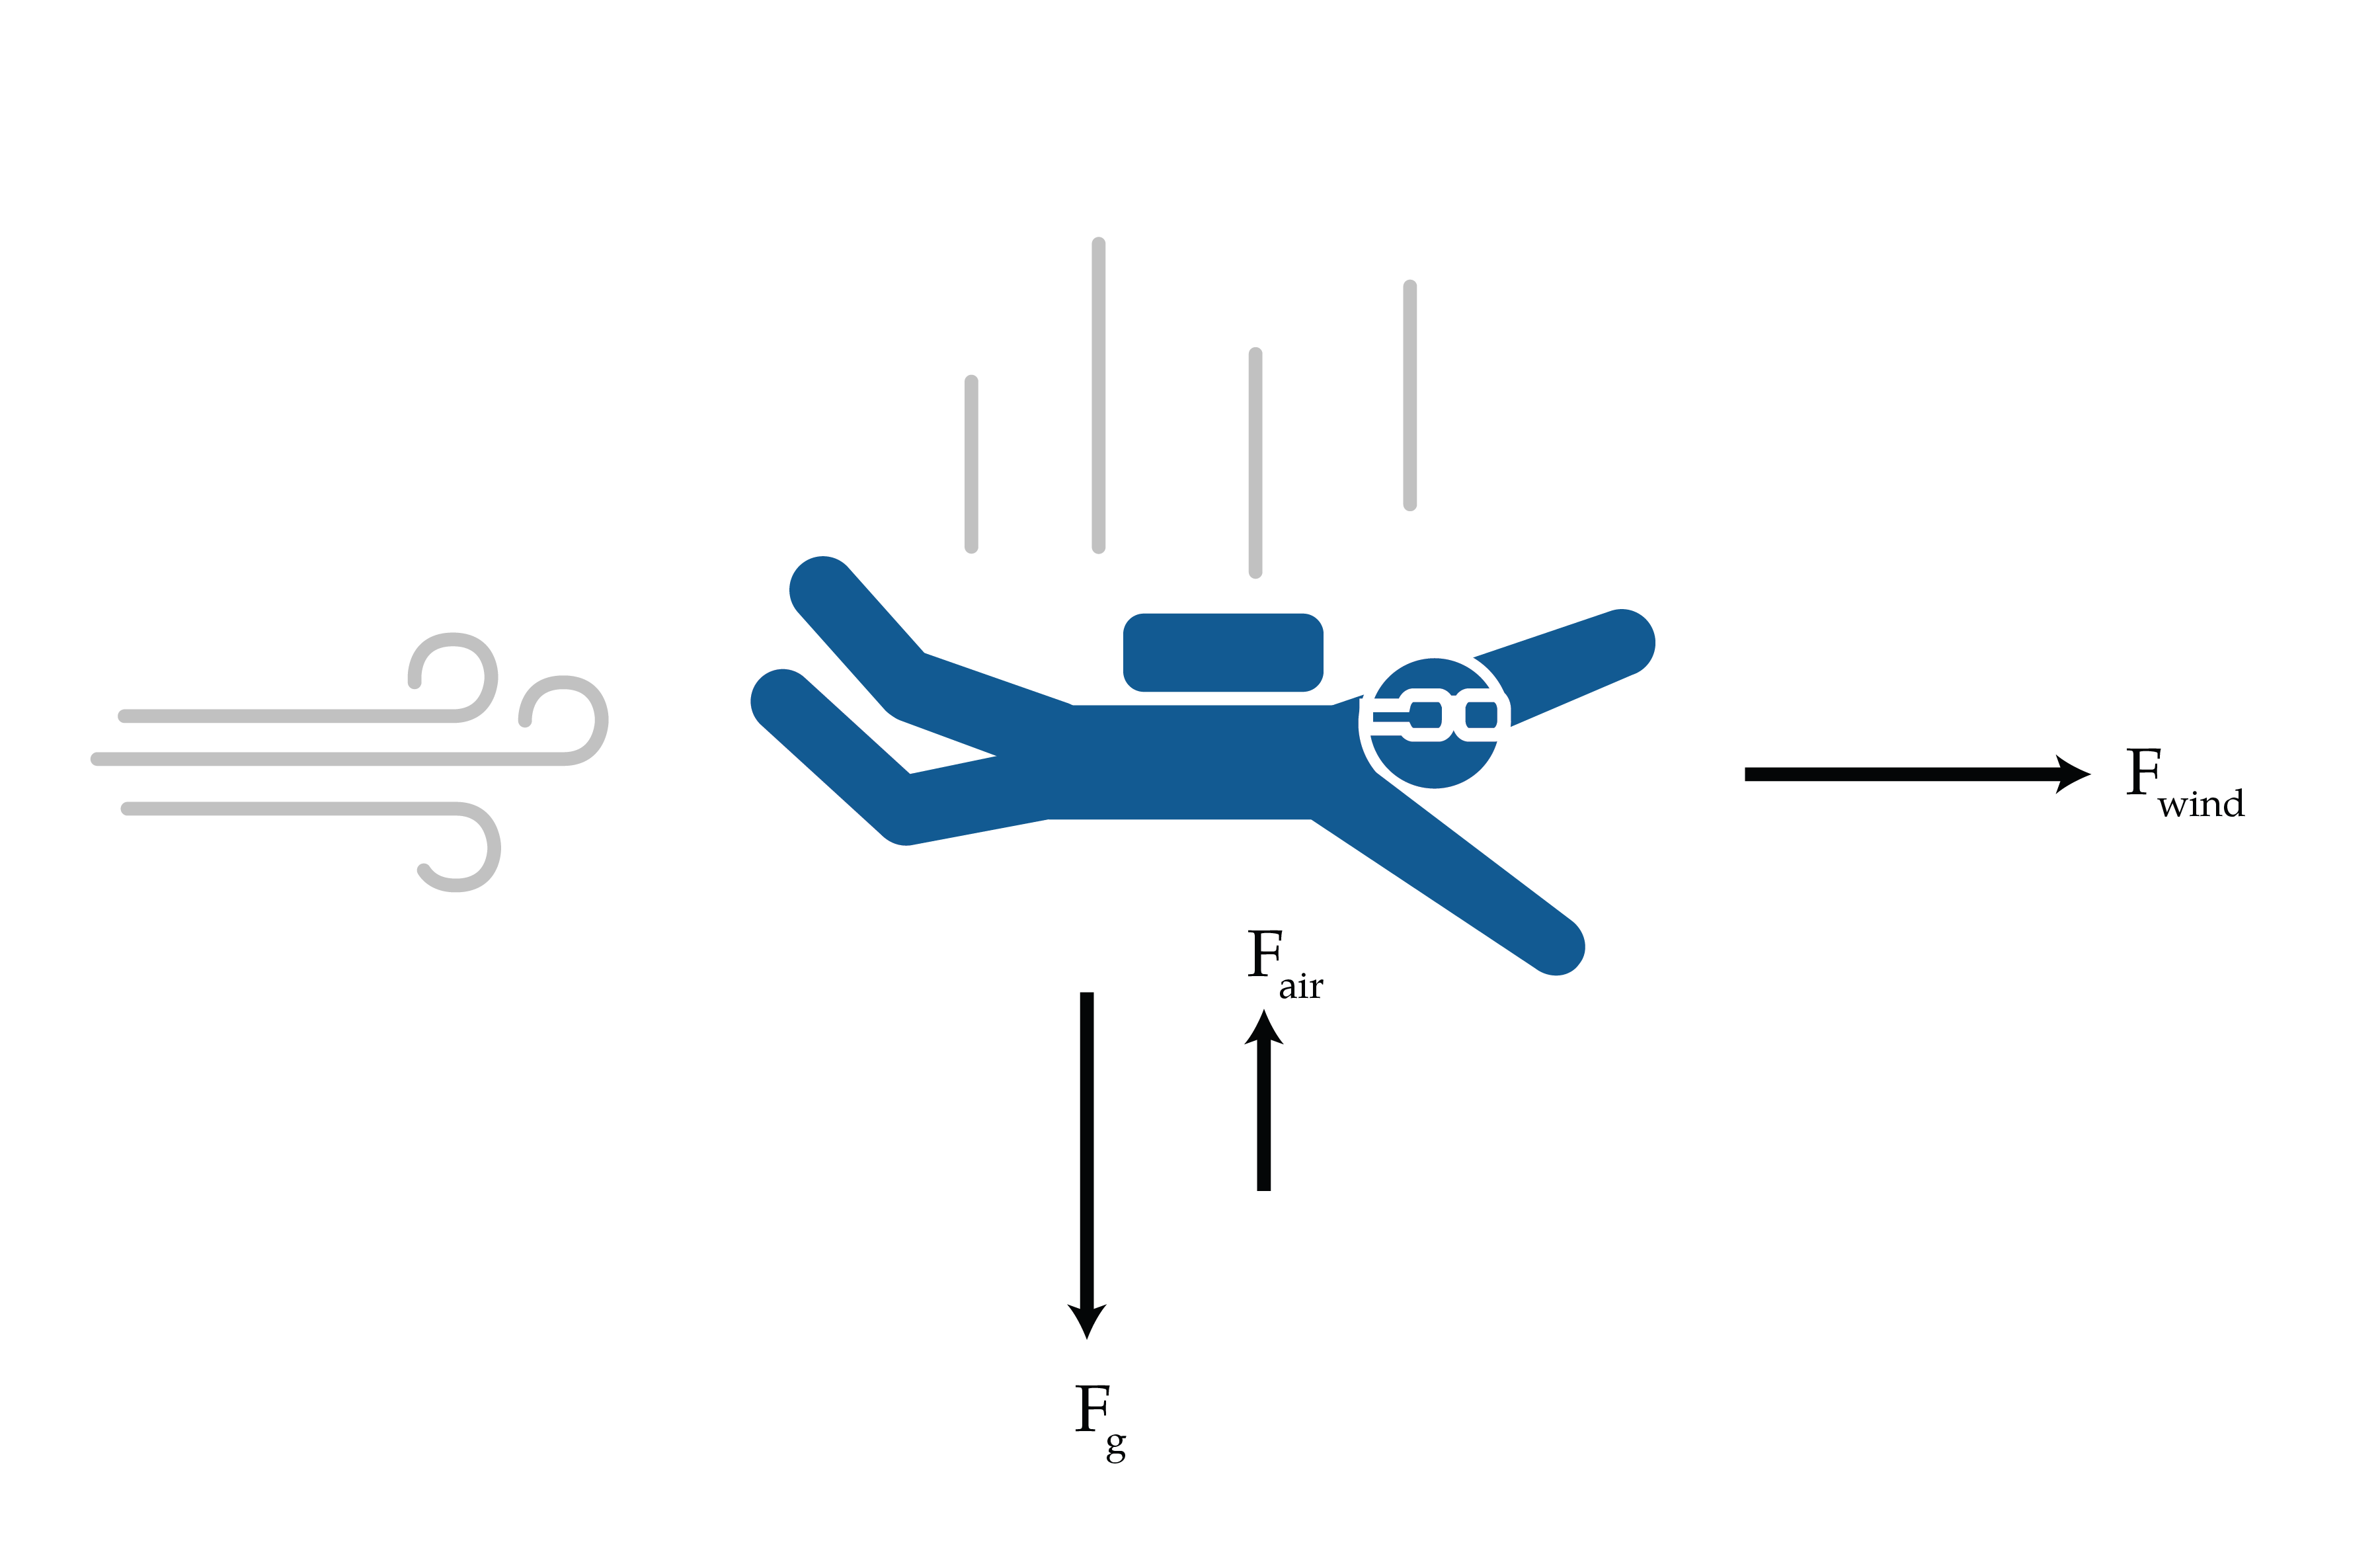
\includegraphics[width=1\textwidth]{skydiver.png}

To figure out the net force (which will tell us how we will accelerate), we 
will need to add these forces together. To do this, we need to learn to do 
math with vectors.

\section{Adding Vectors}

A vector is typically represented as a list of numbers, with each
number representing a particular dimension. For example, if you are
creating a 3-dimensional vector representing a force, it will have
three numbers representing the amount of force in each of the three
axes. For example, if a force of one newton is in the direction of the
$x$-axis, you might represent the vector as $v = [1, 0, 0]$. 
Another vector might be $u = [0.5, 0.9, 0.7]$ \index{vectors!adding}. You can 
see examples of 2-dimensional and 3-dimensional vectors in figures 
\ref{fig:2d_vectors} and \ref{fig:3d_vectors}. 

\begin{figure}[htbp]
    \centering
    \begin{tikzpicture}
        \begin{axis}[xmin = -0.5, ymin = -0.5, xmax = 6, ymax = 6, 
        axis lines = center, xlabel = $x$, ylabel = $y$]
            \draw[blue, thick, -latex](0, 0) -- (2, 3) node[right, black, 
            font = \scriptsize] {$\textbf{u} = \left[ 2, 3 \right]$};
            \draw[blue, thick, -latex] (0, 0) -- (4, 1) node[above, black, 
            font = \scriptsize] {$\textbf{v} = \left[ 4, 1 \right]$};
        \end{axis}
    \end{tikzpicture}
    \caption{2-dimensional vectors, \textbf{u} and \textbf{v}}
    \label{fig:2d_vectors}
\end{figure}

\begin{figure}[htbp]
\centering
\tdplotsetmaincoords{80}{130} 
\begin{tikzpicture} [scale=4, tdplot_main_coords, axis/.style={->,black}, 
vector/.style={-stealth,blue,very thick}, 
vector guide/.style={dashed,black}]

%standard tikz coordinate definition using x, y, z coords
\coordinate (O) at (0,0,0);

%draw axes
\draw[axis] (0,0,0) -- (1.5,0,0) node[anchor=north east]{$x$};
\draw[axis] (0,0,0) -- (0,0.9,0) node[anchor=north west]{$y$};
\draw[axis] (0,0,0) -- (0,0,0.9) node[anchor=south]{$z$};

%draw a vector from O to P
\draw[vector] (O) -- (1,0,0);
\draw[vector] (O) -- (0.5,0.9,0.7);
\draw (0.2,0.0,0.05) node[left] {v};
\draw (0.2,0.35,0.3) node[right] {u};

\draw[vector guide] (0.5,0,0) -- (0.5,0.9,0);
\draw[vector guide] (0.0,0.9,0) -- (0.5,0.9,0);
\draw[vector guide] (0.5,0.9,0) -- (0.5,0.9,0.7);
\end{tikzpicture}
\caption{3-dimensional vectors, \textbf{u} and \textbf{v}}
\label{fig:3d_vectors}
\end{figure}


Thinking visually, when we add to vectors, we put the starting point second 
vector at the ending point of the first vector. This is illustrated for 
2-dimensional vectors in figure \ref{fig:2d_add} and for 3-dimensional vectors 
in figure \ref{fig:3d_add}. 

\begin{figure}[htbp]
    \centering
    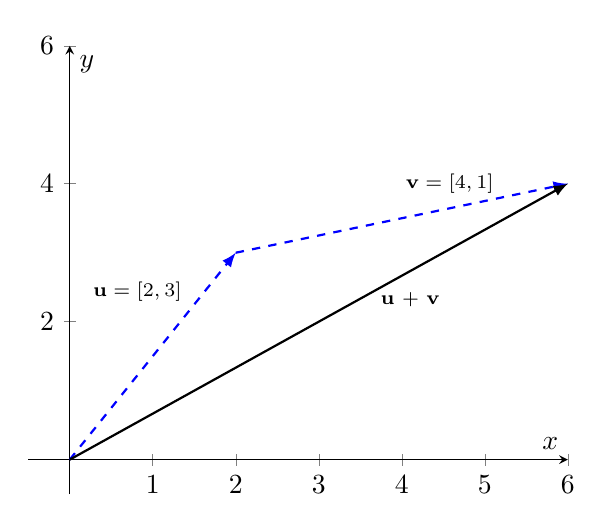
\begin{tikzpicture}
        \begin{axis}[xmin = -0.5, ymin = -0.5, xmax = 6, ymax = 6, 
        axis lines = center, xlabel = $x$, ylabel = $y$, clip = false]
           \draw[blue, thick, -latex, dashed](0, 0) -- (2, 3) node[above, 
           xshift = -1.25cm, yshift = -0.75cm, black, font = \scriptsize] {
           $\textbf{u} = \left[ 2, 3 \right]$}; 
           \draw[blue, thick, -latex, dashed] (2, 3) -- (6, 4) node[above, 
           xshift = -1.5cm, yshift = -0.25 cm, black, font = \scriptsize] {
           $\textbf{v} = \left[ 4, 1 \right]$};
           \draw[black, thick, -latex] (0, 0) -- (6, 4) node[below, black, 
           xshift = -2cm, yshift = -1.25cm, font = \scriptsize] {\textbf{u} + 
           \textbf{v}};
        \end{axis}
    \end{tikzpicture}
    \caption{A visual representation of adding 2-dimensional vectors, 
    \textbf{u} and \textbf{v}}
    \label{fig:2d_add}
\end{figure}

\begin{figure}[htbp]
\centering
\tdplotsetmaincoords{80}{130} 
\begin{tikzpicture} [scale=4, tdplot_main_coords, axis/.style={->,black}, 
light vector/.style={-stealth,dashed,very thick, blue}, 
vector/.style={-stealth,black,very thick}, 
vector guide/.style={dashed,black}]

%standard tikz coordinate definition using x, y, z coords
\coordinate (O) at (0,0,0);

%draw axes
\draw[axis] (0,0,0) -- (1.5,0,0) node[anchor=north east]{$x$};
\draw[axis] (0,0,0) -- (0,0.9,0) node[anchor=north west]{$y$};
\draw[axis] (0,0,0) -- (0,0,0.9) node[anchor=south]{$z$};

%draw a vector from O to P
\draw[light vector] (0,0,0) -- (0.5,0.9,0.7);
\draw[light vector] (0.5, 0.9, 0.7) -- (1.5, 0.9, 0.7);
\draw[vector] (0,0,0) -- (1.5,0.9,0.7) node[left] {u + v};
\draw (0.7,0.9,0.75) node[left] {v};
\draw (0.2,0.35,0.3) node[right] {u};

\draw[vector guide] (0.5,0,0) -- (0.5,0.9,0);
\draw[vector guide] (0.0,0.9,0) -- (0.5,0.9,0);
\draw[vector guide] (0.5,0.9,0) -- (0.5,0.9,0.7);
\draw[vector guide] (0.5,0.9,0) -- (1.5,0.9,0.0);
\draw[vector guide] (1.5,0.9,0.0) -- (1.5,0.9,0.7);
\draw[vector guide] (1.5,0.0,0.0) -- (1.5,0.9,0.0);

\end{tikzpicture}
\caption{A visual representation of adding 3-dimensional vectors, \textbf{u} 
and \textbf{v}}
\label{fig:3d_add}
\end{figure}

If you know the vectors, you will just add them element-wise:

$$ u + v = [0.5, 0.9, 0.7] + [1.0, 0.0, 0.0] = [1.5, 0.9. 0.7] $$

These vectors have 3 components, so we say they are \newterm{3-dimensional}. 
Vectors can have any number of components. For example, the vector
 $[-12.2, 3, \pi, 10000]$ is 4-dimensional.

 You can only add two vectors if they have the same dimension.

 $$ [12, -4] + [-1, 5] = [11,1] $$

 Addition is commutative; if you have two vectors $a$ and $b$, then
 $a + b$ is the same as $b + a$.

 Addition is also associative: If you have three vectors $a$, $b$, and $c$,
 it doesn't matter which order you add them in. 
 That is, $a + (b + c) = (a + b) + c$.

 A 1-dimensional vector is just a number. We say it is a 
 \newterm{scalar}, not a vector.

 \begin{Exercise}[title={Adding vectors}, label=adding_vectors]
Add the following vectors:
\begin{itemize}
    \item $[1, 2, 3] + [4, 5, 6]$
    \item $[-1, -2, -3, -4] + [4, 5, 6, 7]$
    \item $[\pi, 0, 0] + [0, \pi, 0] + [0, 0, \pi]$
\end{itemize}
\end{Exercise}
\begin{Answer}[ref=adding_vectors]
    \begin{itemize}
        \item $[1, 2, 3] + [4, 5, 6] = [5, 7, 9]$
        \item $[-1, -2, -3, -4] + [4, 5, 6, 7] = [3, 3, 3, 3]$
        \item $[\pi, 0, 0] + [0, \pi, 0] + [0, 0, \pi] = [\pi, \pi, \pi]$ 
    \end{itemize}
\end{Answer}

    \begin{Exercise}[title={Adding Forces}, label=adding_forces]
        You are adrift in space, near two different stars. 
        The gravity of one star is pulling you towards it with a 
        force of $[4.2, 5.6, 9.0]$ newtons.
        The gravity of the other star is pulling you towards it with
        a force of $[-100.2, 30.2, -9.0]$ newtons. What is the net force?
        \end{Exercise}
        \begin{Answer}[ref=adding_forces]
            To get the net force, you add the two forces:

            $$F = [4.2, 5.6, 9.0] + [-100.2, 30.2, -9.0] = [-96, 35.8, 0.0] 
            \text{ newtons}$$
   
\end{Answer}

\section{Multiplying a vector with a scalar}

It is not uncommon to multiply a vector by a scalar. For example, a rocket engine
might have a force vector $v$. If you fire 9 engines in the exact same direction,
the resulting force vector would be $9v$.\index{vectors!multipying by a scalar}

Visually, when we multiply a vector $u$ by a scalar $a$, we get a new vector that
goes in the same direction as $u$ but has a magnitude $a$ times as long as 
$u$. A visual is presented in figure \ref{fig:multiply}.


\begin{figure}
\centering
\tdplotsetmaincoords{80}{130} 
\begin{tikzpicture} [scale=3, tdplot_main_coords, axis/.style={->,black}, 
vector/.style={-stealth,blue,very thick}, 
vector guide/.style={dashed,black}]

%standard tikz coordinate definition using x, y, z coords
\coordinate (O) at (0,0,0);

%draw axes
\draw[axis] (0,0,0) -- (1.6,0,0) node[anchor=north east]{$x$};
\draw[axis] (0,0,0) -- (0,2.8,0) node[anchor=north west]{$y$};
\draw[axis] (0,0,0) -- (0,0,1.9) node[anchor=south]{$z$};

%draw a vector from O to P
\draw[vector] (O) -- (0.5,0.9,0.7);
\draw (0.2,0.35,0.3) node[right] {$u$};

\draw[vector] (O) -- (1.5,2.7,2.1) node[right] {$3u$};


\draw[vector guide] (0.5,0,0) -- (0.5,0.9,0);
\draw[vector guide] (0.0,0.9,0) -- (0.5,0.9,0);
\draw[vector guide] (0.5,0.9,0) -- (0.5,0.9,0.7);

\draw[vector guide] (1.5,0,0) -- (1.5,2.7,0);
\draw[vector guide] (0.0,2.7,0) -- (1.5,2.7,0);
\draw[vector guide] (1.5,2.7,0) -- (1.5,2.7,2.1);
\end{tikzpicture}
\caption{To multiply vectors, the vector gets stretched in the same direction $a$ amount}
\label{fig:multiply}
\end{figure}


When you multiply a vector by a scalar, you simply multiply each of the 
components by the scalar:

$$ 3 \times [0.5, 0.9, 0.7] = [1.5, 2.7, 3.6] $$

\begin{Exercise}[title={Multiplying a vector and a scalar}, label=mult_scalar]
    Simplify the following expressions:
    \begin{itemize}
        \item $2 \times [1, 2, 3]$
        \item $[-1, -2, -3, -4] \times -2$
        \item $\pi[\pi, 2\pi, 3\pi]$
    \end{itemize}
    \end{Exercise}
    \begin{Answer}[ref=mult_scalar]
        \begin{itemize}
            \item $2 \times [1, 2, 3] = [2, 4, 6]$
            \item $[-1, -2, -3, -4] \times -3 = [3, 6, 9, 12]$
            \item $\pi[\pi, 2\pi, 3\pi]  = \pi^2, 2\pi^2, 3\pi^2]$ 
        \end{itemize}
    \end{Answer}

Note that when you multiply a vector times a negative number, the new vector 
points in the opposite direction (see figure \ref{fig:negative}).

\begin{figure}[htbp]
\centering
\tdplotsetmaincoords{80}{130} 
\begin{tikzpicture} [scale=5, tdplot_main_coords, axis/.style={->,black}, 
vector/.style={-stealth,blue,very thick}, 
vector guide/.style={dashed,black}]

%standard tikz coordinate definition using x, y, z coords
\coordinate (O) at (0,0,0);

%draw axes
\draw[axis] (0,0,0) -- (0.55,0,0) node[anchor=north east]{$x$};
\draw[axis] (0,0,0) -- (0,0.95,0) node[anchor=north west]{$y$};
\draw[axis] (0,0,0) -- (0,0,0.6) node[anchor=south]{$z$};

%draw a vector from O to P
\draw[vector] (O) -- (0.5,0.9,0.7);
\draw (0.2,0.36,0.3) node[right] {$u$};

\draw[vector, red] (O) -- (-0.25,-0.45,-0.35) node[right] {$(-0.5)u$};

\draw[vector guide] (0.5,0,0) -- (0.5,0.9,0);
\draw[vector guide] (0.0,0.9,0) -- (0.5,0.9,0);
\draw[vector guide] (0.5,0.9,0) -- (0.5,0.9,0.7);

\draw[vector guide] (-0.25,0,0) -- (-0.25,-0.45,0);
\draw[vector guide] (0,0,0) -- (-0.25,0,0);
\draw[vector guide] (0.0,-0.45,0) -- (-0.25,-0.45,0);
\draw[vector guide] (0,0,0) -- (0,-0.45,0);

\draw[vector guide] (-.25,-0.45,0) -- (-0.25,-0.45,-0.35);
\end{tikzpicture}
\caption{Multiplying a vector by a negative number reverses the direction of 
the vector.}
\label{fig:negative}
\end{figure}

\section{Vector Subtraction}

As you might guess, when you subtract one vector from another, 
you just do element-wise subtraction:\index{vectors!subtraction}

$$[4,2,0] - [3,-2, 9] = [1, 4, -9]$$

So, $u - v = u + (-1v)$.

Visually, you reverse the one that is being subtracted (see figure 
\ref{fig:subtract}):

\begin{figure}[htbp]
\centering
\tdplotsetmaincoords{80}{130} 
\begin{tikzpicture} [scale=5, tdplot_main_coords, axis/.style={->,black}, 
light vector/.style={-stealth,dashed,very thick, black}, 
vector/.style={-stealth,blue,very thick}, 
vector guide/.style={dashed,black}]

%standard tikz coordinate definition using x, y, z coords
\coordinate (O) at (0,0,0);

%draw axes
\draw[axis] (0,0,0) -- (0.55,0,0) node[anchor=north east]{$x$};
\draw[axis] (0,0,0) -- (0,1.0,0) node[anchor=north west]{$y$};
\draw[axis] (0,0,0) -- (0,0,0.75) node[anchor=south]{$z$};

%draw a vector from O to P
\draw[light vector] (0,0,0) -- (0.5,0.9,0.7);
\draw[light vector] (0.5, 0.9, 0.7) -- (-0.5, 0.9, 0.7);
\draw[vector] (0,0,0) -- (-0.5,0.9,0.7) node[right] {u - v};
\draw (0.1,0.9,0.75) node[left] {-v};
\draw (0.29,0.34,0.32) node[right] {u};

\draw[vector guide] (0.5,0,0) -- (0.5,0.9,0);
\draw[vector guide] (0.0,0.9,0) -- (0.5,0.9,0);
\draw[vector guide] (0.5,0.9,0) -- (0.5,0.9,0.7);
\draw[vector guide] (0.5,0.9,0) -- (-0.5,0.9,0.0);
\draw[vector guide] (-0.5,0.9,0.0) -- (-0.5,0.9,0.7);
\draw[vector guide] (-0.5,0.0,0.0) -- (-0.5,0.9,0.0);
\draw[vector guide] (0,0.0,0.0) -- (-0.5,0.0,0.0);

\end{tikzpicture}
\caption{To subtract a vector, you reverse it, then add the reversed vector.}
\label{fig:subtract}
\end{figure}

\section{Magnitude of a Vector}

The \newterm{magnitude} of a vector is just its length. We write the 
magnitude of a vector $v$ as $|v|$.\index{vectors!magnitude of}

We compute the magnitude using the pythagorean theorem.  If $v = [3,4,5]$, 
then

\begin{equation*}
    |v| = \sqrt{3^2 + 4^2 + 5^2} = \sqrt{50} \approx 7.07
\end{equation*}

(You might notice that the notation for the magnitude is exactly like the 
notation for absolute value. If you think of a scalar as a 1-dimensional 
vector, the absolute value and the magnitude are the same. For example, the 
absolute value of -5 is 5.  If you take the magnitude of the one-dimensional 
vector $[-5]$,you get $\sqrt{25} = 5$.)

Where does this equation come from? Consider a 2-dimensional vector, 
$\textbf{v} = \left[ 3, 4 \right]$. This means the the vector represents 3 
units in the $x$-direction, and 4 units in the $y$-direction. We can then 
visualize a right triangle, with the vector being the hypotenuse and the legs 
being the $x$- and $y$-components of the vector (see figure 
\ref{fig:triangle}). As you recall, the length of the hypotenuse of a right 
triangle is the square root of the sum of the squares of the legs. That is:
$$c = \sqrt{a^2 + b^2}$$

Where $c$ is the length of the hypotenuse and $a$ and $b$ are the lengths of 
the legs. 

\begin{figure}
    \centering
    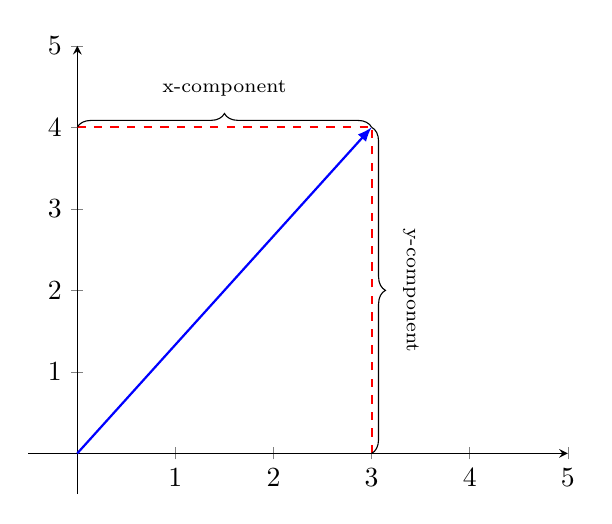
\begin{tikzpicture}
        \begin{axis}[axis lines = center, xmin = -0.5, ymin = -0.5, xmax = 5, 
        ymax = 5, clip = false]
            \draw[blue, thick, -latex] (0, 0) -- (3, 4);
            \draw[red, dashed, thick] (0, 4) -- (3, 4);
            \draw[red, dashed, thick] (3, 0) -- (3, 4);
            \draw[decorate, decoration = {brace, amplitude = 5pt}] (0, 4) -- 
            (3, 4) node[midway, font = \scriptsize, yshift = 0.5cm] 
            {x-component};
            \draw[decorate, decoration = {brace, amplitude = 5pt, mirror}] 
            (3, 0) -- (3, 4) node[midway, font = \scriptsize, rotate = -90, 
            yshift = 0.5cm] {y-component};
        \end{axis}
    \end{tikzpicture}
    \caption{The magnitude of a vector can be thought of as the length of a 
    hypotenuse of a right triangle.}
    \label{fig:triangle}
\end{figure}

We won't prove it here, but this method holds for higher-dimension vectors as well. 

\begin{mdframed}[style = important, frametitle = {Magnitude of Vectors}]
For an $n$-dimensional vector, $\textbf{v} = \left[ x_1, x_2, x_3, \cdots, x_n 
\right]$, the magnitude of the vector is given by:
$$\left| \textbf{v} \right| = \sqrt{x_1^2 + x_2^2 + x_3^2 + \cdots + x_n^2}$$
\end{mdframed}

Notice that if you scale up a vector, its magnitude scales by the same amount. 
For example:

\begin{equation*}
|7[3,4,5]| = 7 \sqrt{50} \approx 7 \times 7.07    
\end{equation*}

Here is why that is true. Suppose we have a vector, $\textbf{u} = \left[a, b, 
c \right]$. Then the magnitude of $\textbf{u}$ is given by:
$$\left| \textbf{u} \right| = \sqrt{a^2 + b^2 + c^2}$$

If we scale \textbf{u} to create \textbf{v} such that $\textbf{v} = k 
\textbf{u} = \left[ ka, kb, kc \right]$, where $k$ is some constant. Then the 
magnitude of \textbf{v} is given by:
$$\left| \textbf{v} \right| = \sqrt{\left( ka \right)^2 + \left( kb \right)^2 
+ \left( kc \right)^2}$$

We can expand and simplify this equation:
$$\left| \textbf{v} \right| = \sqrt{k^2 a^2 + k^2 b^2 + k^2 c^2}$$
$$\left| \textbf{v} \right| = \sqrt{k^2 \left( a^2 + b^2 + c^2 \right)}$$
$$\left| \textbf{v} \right| = \left( \sqrt{k^2} \right) \sqrt{a^2 + b^2 + 
c^2}$$
$$\left| \textbf{v} \right| = \left| k \right| \sqrt{a^2 + b^2 + c^2} = 
\left| k \right| \left| \textbf{u} \right|$$

So, if you scale a vector, the magnitude of the resulting vector is the absolute value of the scale factor times the magnitude of the original vector. 

The rule then is: If you have any vector $v$ and any scalar $k$:
\begin{equation*}
    |k v| = |k| |v|
\end{equation*}

\subsection{Unit Vectors}

A \emph{unit vector} is a vector whose magnitude is \(1\).\index{unit vector}
For any non-zero vector \(\mathbf v\), the unit vector pointing in the
same direction is
\[
\vec{\mathbf u}\;=\;\frac{\mathbf v}{\lvert \mathbf v\rvert}.
\]

For example, if \(\mathbf v=[3,4,5]\) then
\[
\lvert\mathbf v\rvert
   \;=\;\sqrt{3^{2}+4^{2}+5^{2}}
   \;=\;\sqrt{50},
\]
so
\[
\vec{\mathbf u}
   \;=\;\frac{1}{\sqrt{50}}\,[3,4,5]
   \;=\;\Bigl[\tfrac{3}{\sqrt{50}},\,
              \tfrac{4}{\sqrt{50}},\,
              \tfrac{5}{\sqrt{50}}\Bigr].
\]

\[
\boxed{\displaystyle
\widehat{\mathbf u}=\frac{\mathbf v}{\lvert\mathbf v\rvert}},\qquad
\lvert\vec{\mathbf u}\rvert=1.
\]



\begin{Exercise}[title={Magnitude of a Vector}, label=vector_mag]
    Find the magnitude of the following vectors:
    \begin{itemize}
        \item $[1, 1, 1]$
        \item $[-5, -5, -5]$ (that is the same as $-5 \times [1, 1, 1]$)
        \item $[3, 4, -4] + [-2, -3, 5]$
    \end{itemize}
    \end{Exercise}
    \begin{Answer}[ref=vector_mag]
        \begin{itemize}
            \item $|[1, 1, 1]| = \sqrt{3} \approx 1.73 $
            \item $|[-5, -5, -5]| = |-5 \times [1,1,1]| = 5 \sqrt{3} \approx 
            8.66$
            \item $|[3, 4, 5] + [-2, -3, -4]| = | [1,1,1] | = \sqrt{3} 
            \approx 1.73$ 
        \end{itemize}
    \end{Answer}

\section{Vectors in Python}

NumPy is a library that allows you to work with vectors in Python. You might 
need to install it on your computer. This is done with \pyfunction{pip}. 
\pyfunction{pip3} installs things specifically for Python 3.
\index{vectors!in python}

\begin{Verbatim}
pip3 install NumPy
\end{Verbatim}

We can think of a vector as a list of numbers.  
There are also grids of numbers known as \newterm{matrices}. NumPy deals with 
both in the same way, so it refers to both of them as arrays.\index{NumPy}

The study of vectors and matrices is known as \newterm{Linear Algebra}. Some 
of the functions we need are in a sublibrary of NumPy called \pyfunction{linalg}. \index{linalg}

As a convention, everyone who uses NumPy, imports it as \textit{np}. \index{np}

Create a file called \filename{first\_vectors.py}:

\begin{Verbatim}
import NumPy as np

# Create two vectors
v = np.array([2,3,4])
u = np.array([-1,-2,3])
print(f"u = {u}, v = {v}")

# Add them
w = v + u
print(f"u + v = {w}")

# Multiply by a scalar
w = v * 3
print(f"v * 3 = {w}")

# Get the magnitude
# Get the magnitude
mv = np.linalg.norm(v)
mu = np.linalg.norm(u)
print(f"|v| = {mv}, |u| = {mu}")
\end{Verbatim}

When you run it, you should see:

\begin{Verbatim}
> python3 first_vectors.py
u = [-1 -2  3], v = [2 3 4]
u + v = [1 1 7]
v * 3 = [ 6  9 12]
|v| = 5.385164807134504, |u| = 3.7416573867739413
\end{Verbatim}

\subsection{Formatting Floats}

The numbers 5.385164807134504 and 3.7416573867739413 are pretty long. You 
probably want them rounded off after a couple of decimal places.

Numbers with decimal places are called \newterm{floats}. In the placeholder 
for your float, you can specify how you want it formatted, including the 
number of decimal places.

Change the last line to look like this:\index{floats!formatting}
\begin{Verbatim}
    print(f"|v| = {mv:.2f}, |u| = {mu:.2f}")
\end{Verbatim}

When you run the code, it will be neatly rounded off to two decimal places:
\begin{Verbatim}
|v| = 5.39, |u| = 3.74
\end{Verbatim}
